\documentclass[12pt]{beamer}

\usepackage{animate}
\usepackage{booktabs}
\usepackage{caption}
\usepackage{subcaption}
\usepackage{graphicx}
\usepackage[backend=bibtex, style=numeric]{biblatex}
    \addbibresource{../references}

\usetheme{metropolis}

\newlength{\imgwidth}
\setlength{\imgwidth}{.95\paperwidth}

\renewcommand{\footnotesize}{\tiny}
\renewcommand*{\bibfont}{\tiny}
\setbeamertemplate{footline}{}
\newsavebox{\largestimage}


\title{Understanding cost variation with clustering}
\author{%
    Henry Wilde \\
    \small{\textit{Supervised by:} Dr Jonathan Gillard and Dr Vincent Knight}
}
\institute{%
    \vfill%
    \centering%
    
\includegraphics[height=.2\paperheight]{img/cu_logo.png}%
    \hspace{5pt}%
    
\includegraphics[height=.2\paperheight]{img/cthb_logo.jpg}
}

\begin{document}

\frame{%
    \maketitle%
}

\frame{\frametitle{The data}
    \begin{itemize}
        \item The Cwm Taf University Health Board
        \item April 2012 through April 2017
        \item 2.4 million patient-episode records with 260 attributes
    \end{itemize}

    \pause%
\begin{table}[htbp]
        \resizebox{\textwidth}{!}{%
            \begin{tabular}{lllrrlllr}
\toprule
&            &              &      Net Cost &   Age (years) &    HRG &
Admission Date &    Discharge Date &  Length of Stay (days) \\
PATIENT ID & SPELL ID & EPISODE ID &              &       &        &             &             &           \\
\midrule
ID\_123456 & M1001 & M1001-1 &   858.14 &  74 &  EA05Z &  2015-05-06 &  2015-05-06 &       0.0 \\
                   & M1211 & M1211-1 &   333.95 &  74 &  FZ38F &  2015-07-15 &  2015-08-01 &      17.0 \\
                   &            & M1211-2 &   706.09 &  74 &  FZ38F &  2015-07-15 &  2015-08-01 &      17.0 \\
                   &            & M1211-3 &  8671.31 &  74 &  RC16Z &  2015-07-15 &  2015-08-01 &      17.0 \\
\bottomrule
\end{tabular}

        }
    \end{table}
}

\section{An overview of the data}
\graphicspath{{img/overview/}}
\frame{\frametitle{An overview}
    \begin{minipage}{.5\linewidth}
        \makebox[\linewidth]{%
            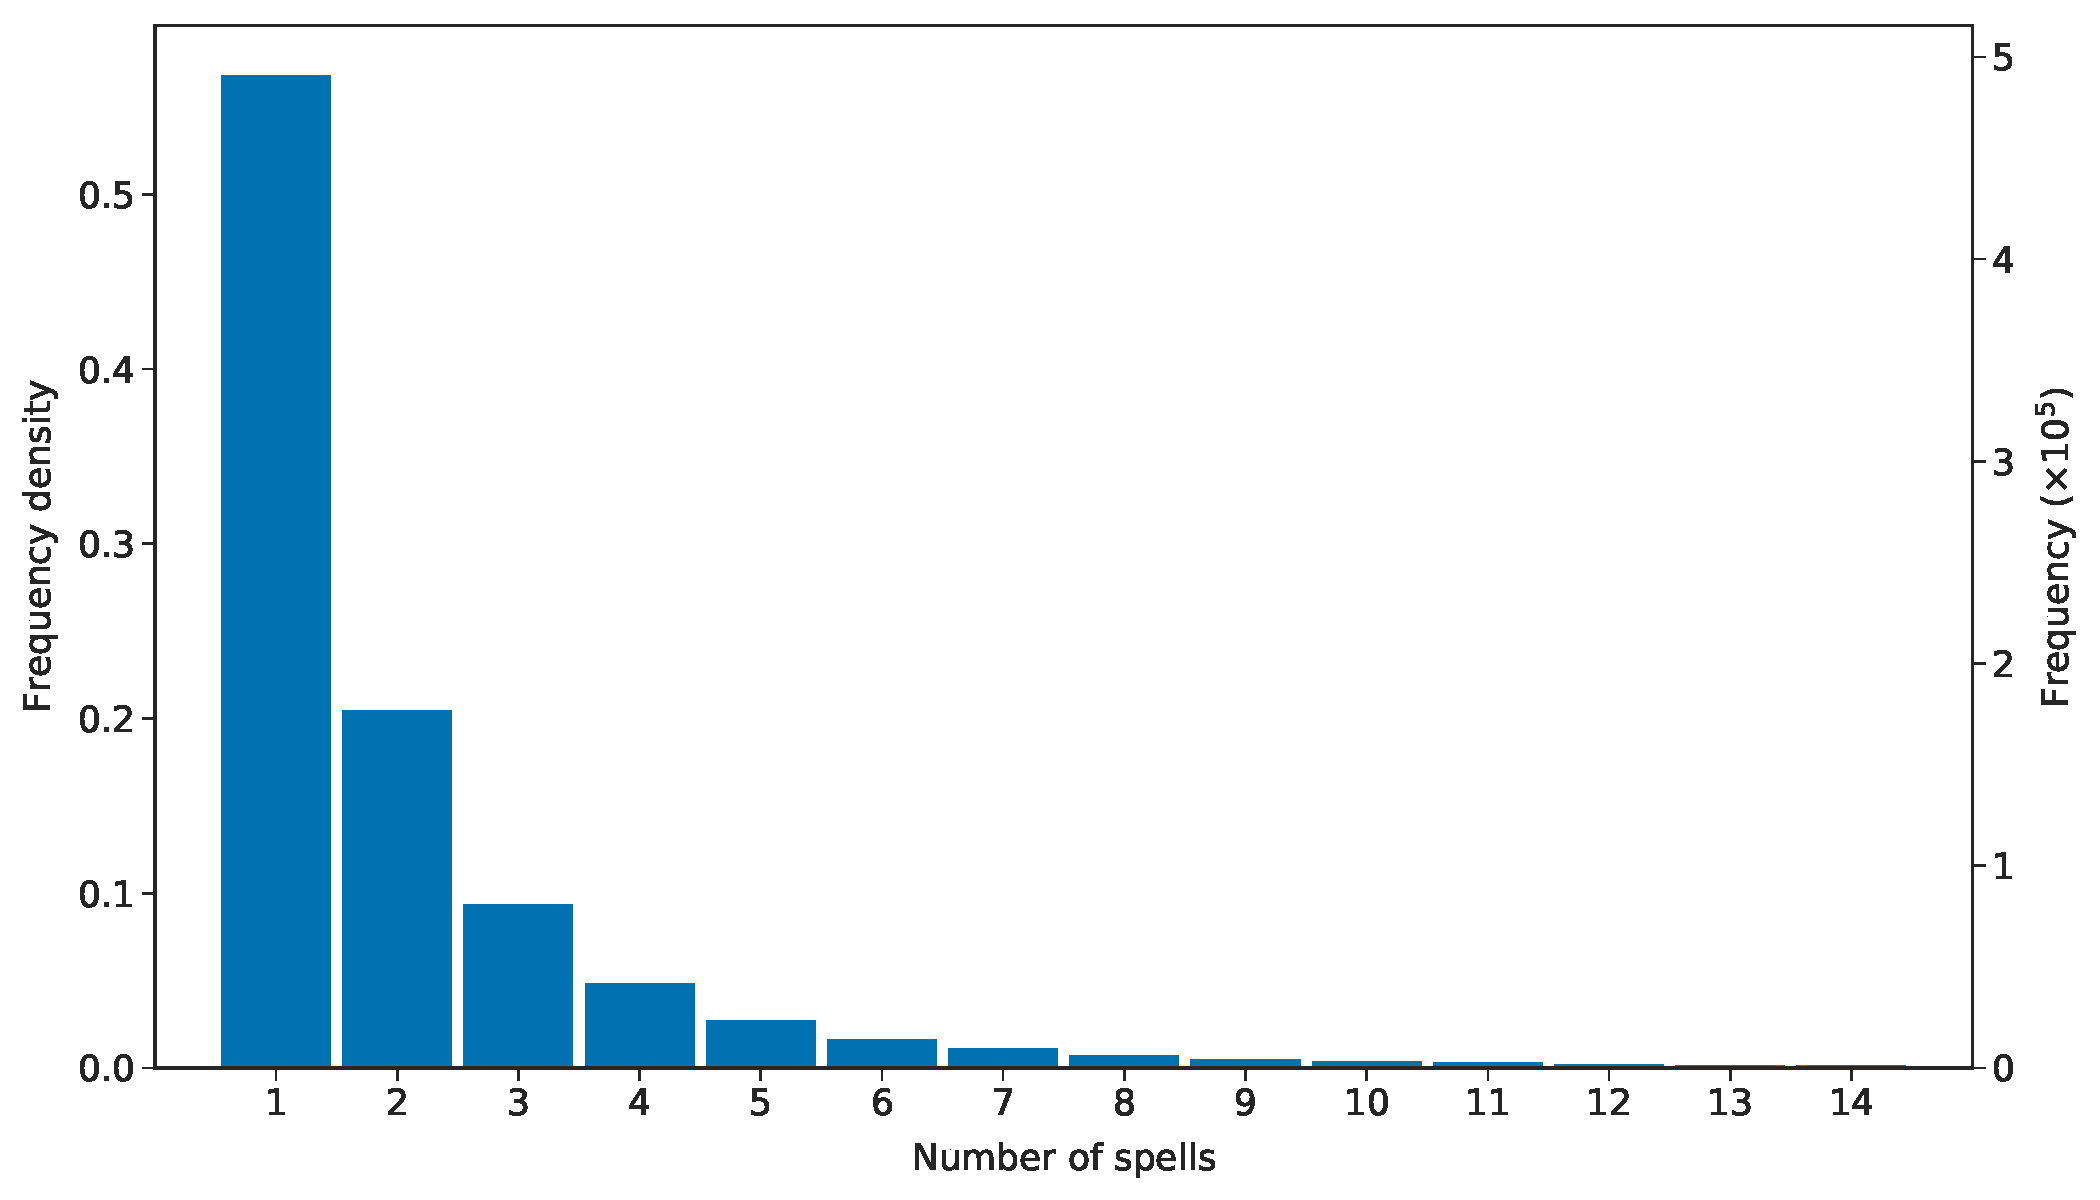
\includegraphics[width=\linewidth]{nspells_bar.pdf}
        }
    \end{minipage}%
    \begin{minipage}{.5\linewidth}
        \makebox[\linewidth]{%
            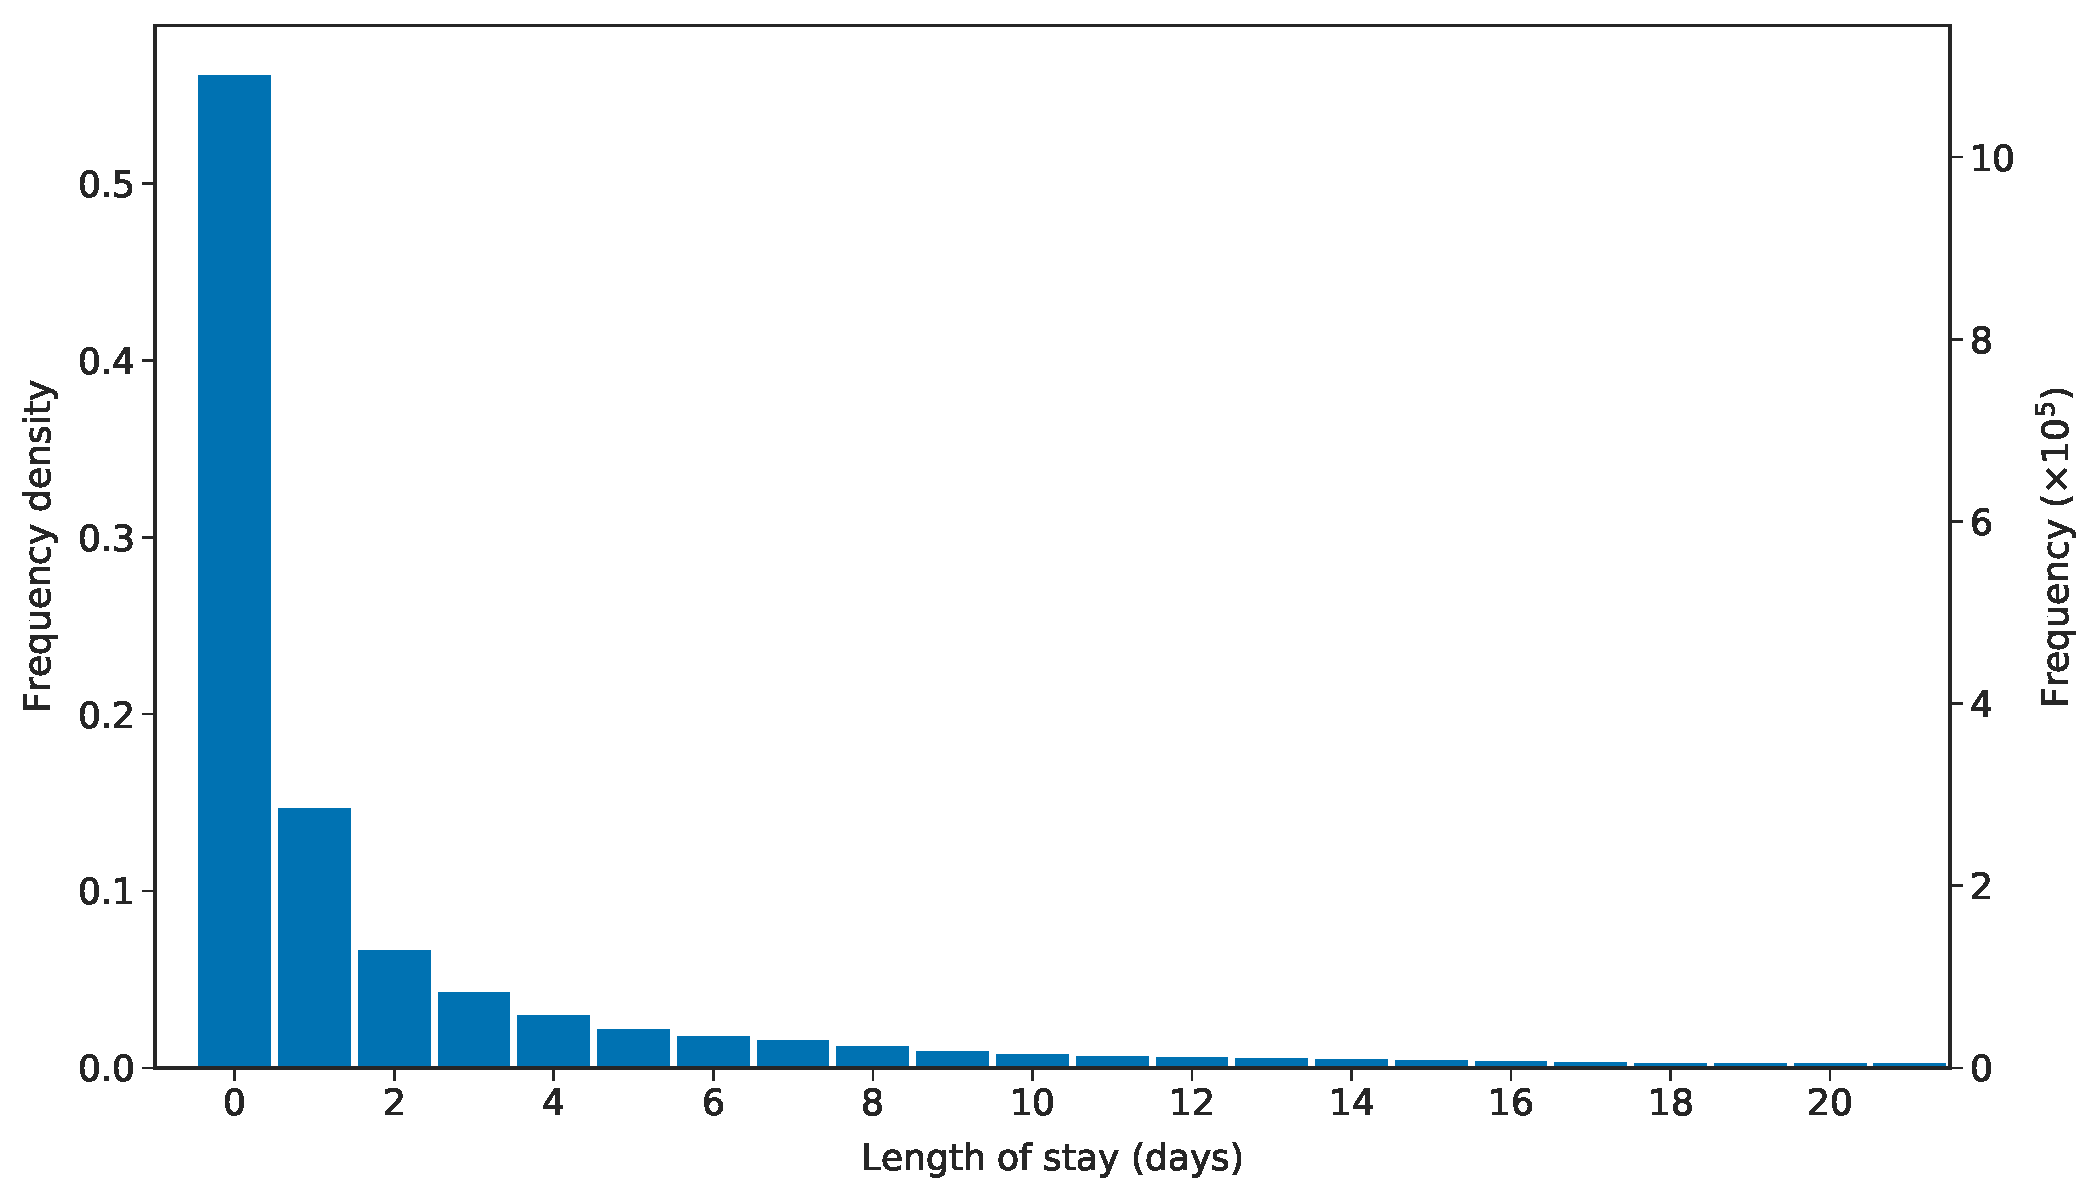
\includegraphics[width=\linewidth]{los_bar.pdf}
        }
    \end{minipage}

    \begin{minipage}{.5\linewidth}
        \makebox[\linewidth]{%
            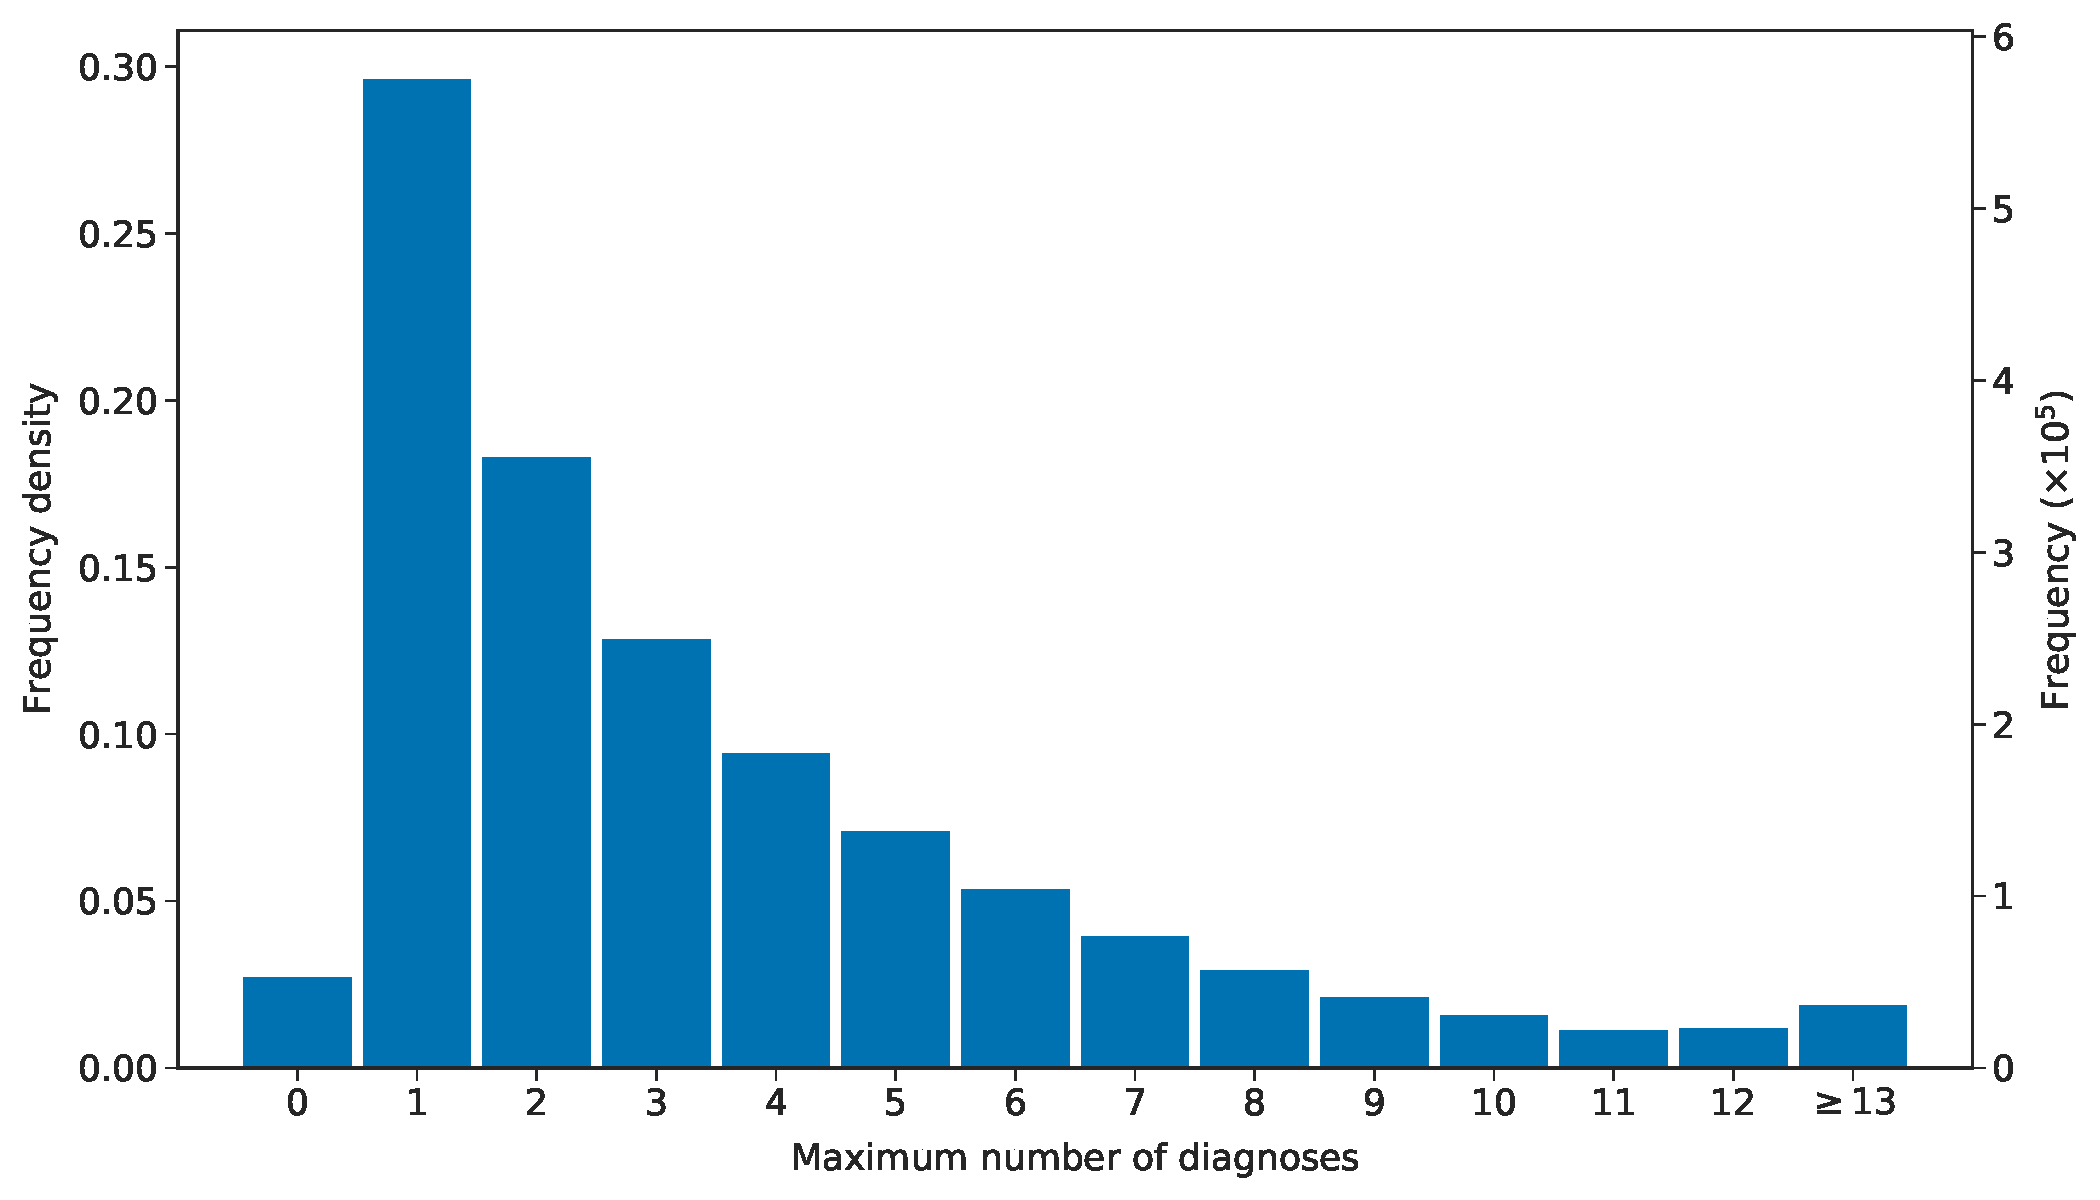
\includegraphics[width=\linewidth]{ndiag_bar.pdf}
        }
    \end{minipage}%
    \begin{minipage}{.5\linewidth}
        \makebox[\linewidth]{%
            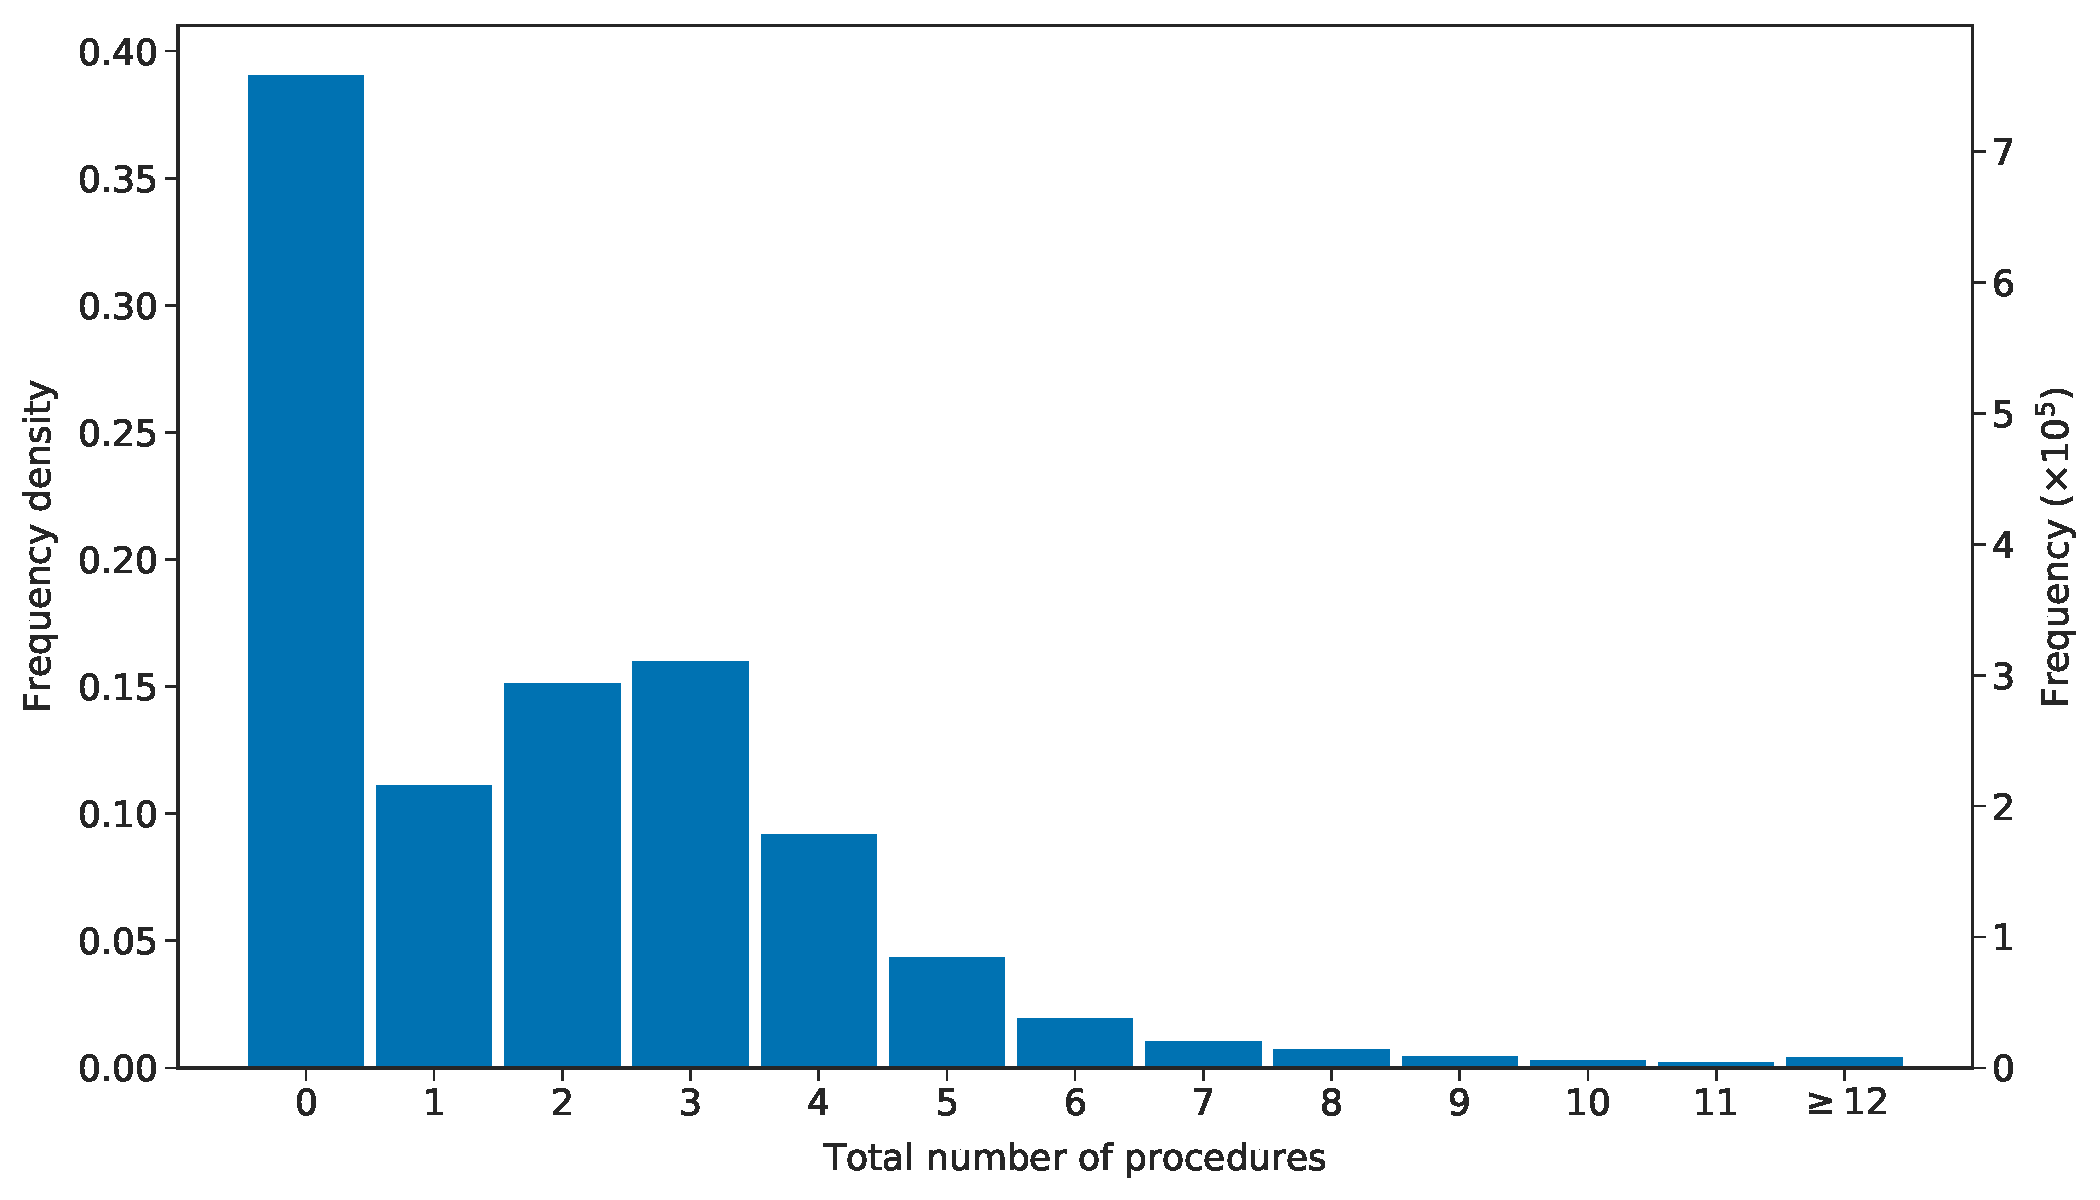
\includegraphics[width=\linewidth]{nproc_bar.pdf}
        }
    \end{minipage}
}

\frame{\frametitle{An overview}
    \makebox[\linewidth]{%
        \begin{minipage}{.8\imgwidth}
            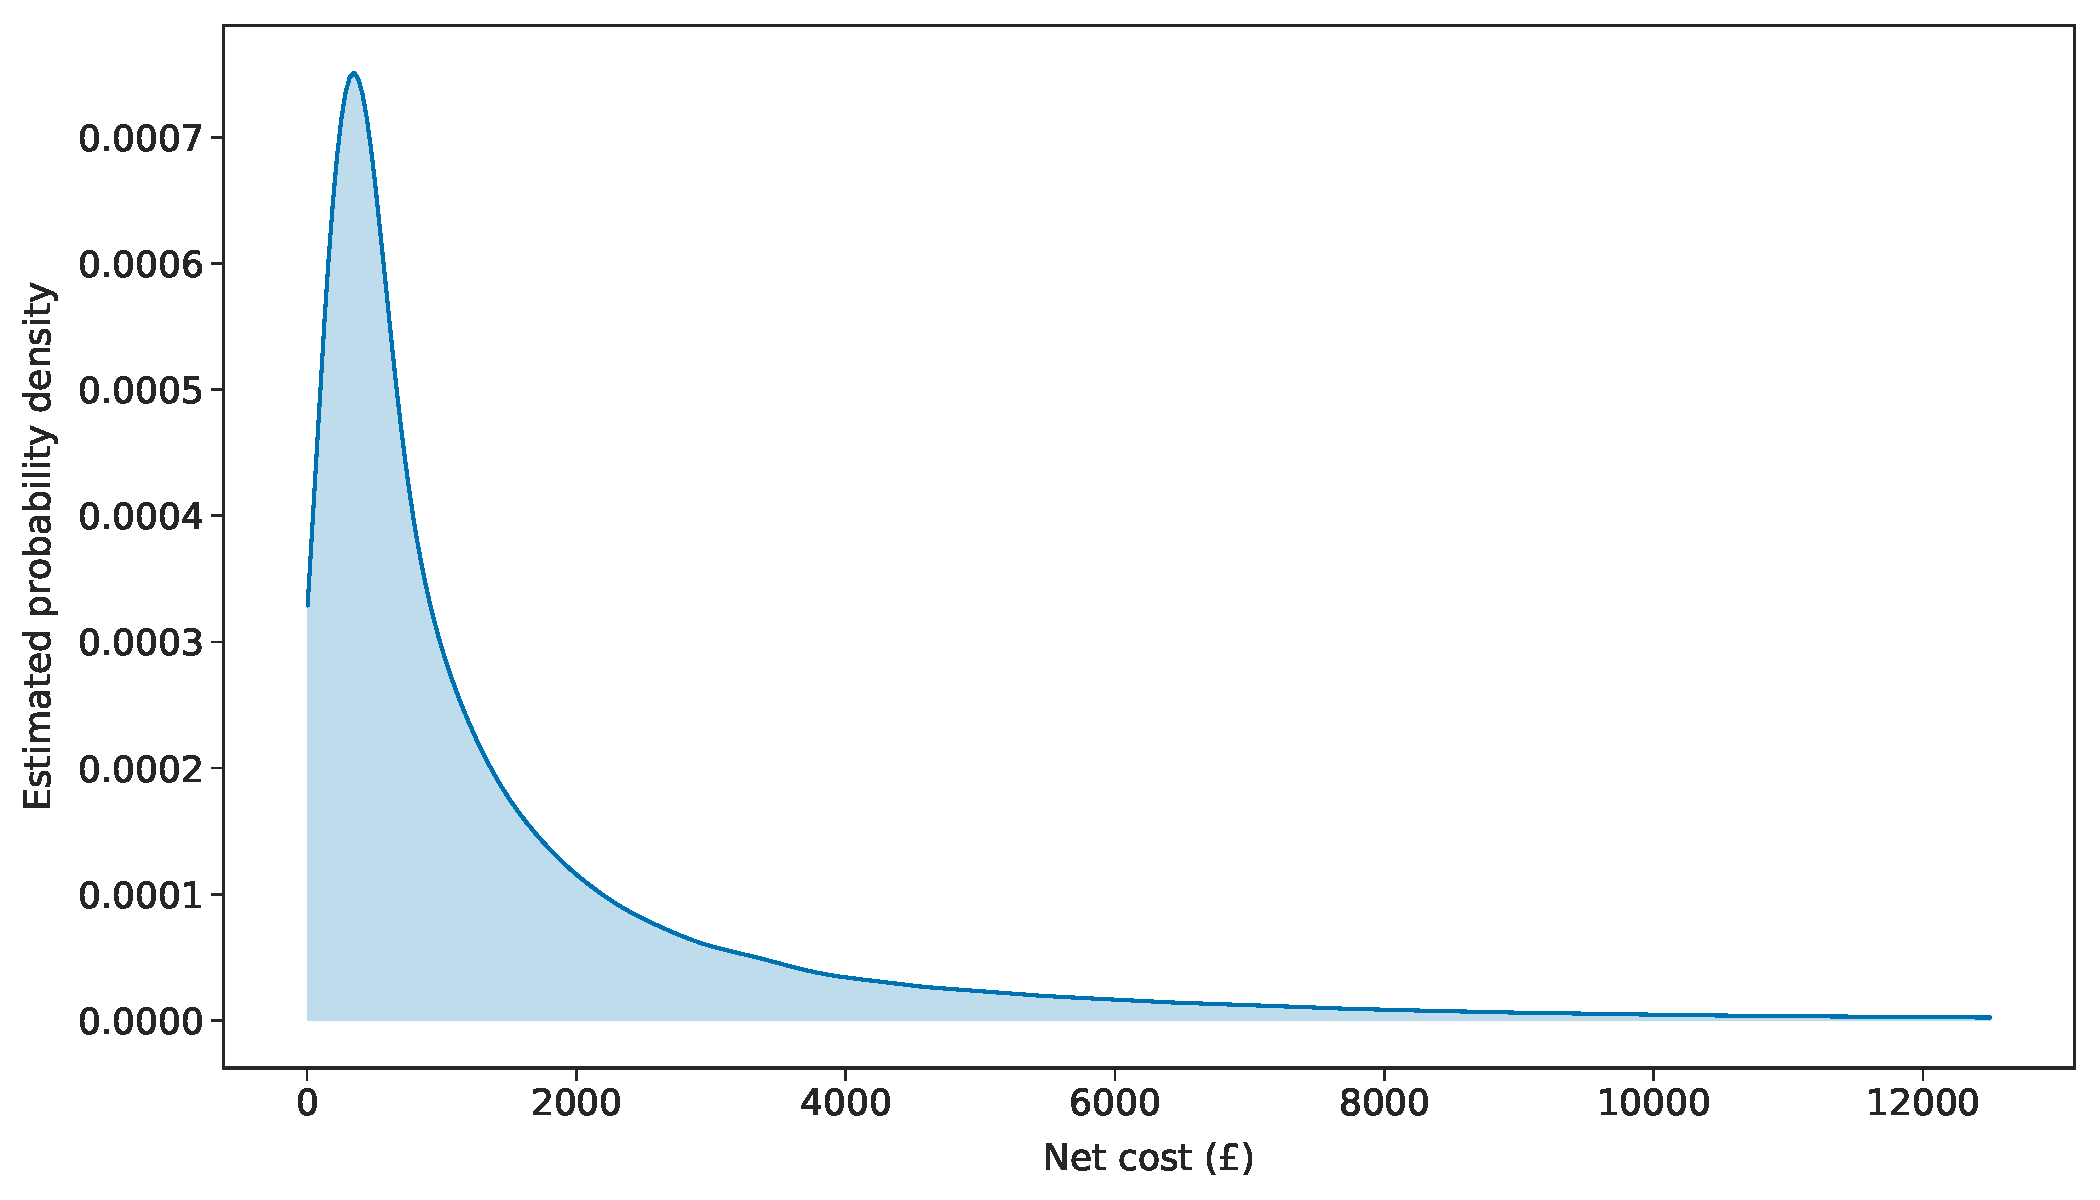
\includegraphics[width=\linewidth]{netcost_kde.pdf}
        \end{minipage}%
        \begin{minipage}{.2\paperwidth}
            \resizebox{\linewidth}{!}{%
                \begin{tabular}{ll}
\toprule
{} &     NetCost \\
\midrule
mean &    1,737.65 \\
std  &    3,160.54 \\
min  &        4.50 \\
1\%   &       62.55 \\
25\%  &      347.07 \\
50\%  &      745.51 \\
75\%  &    1,859.00 \\
95\%  &    6,554.91 \\
99\%  &   14,183.23 \\
max  &  369,168.93 \\
\bottomrule
\end{tabular}

            }
        \end{minipage}
    }
}

\frame{\frametitle{An overview}
    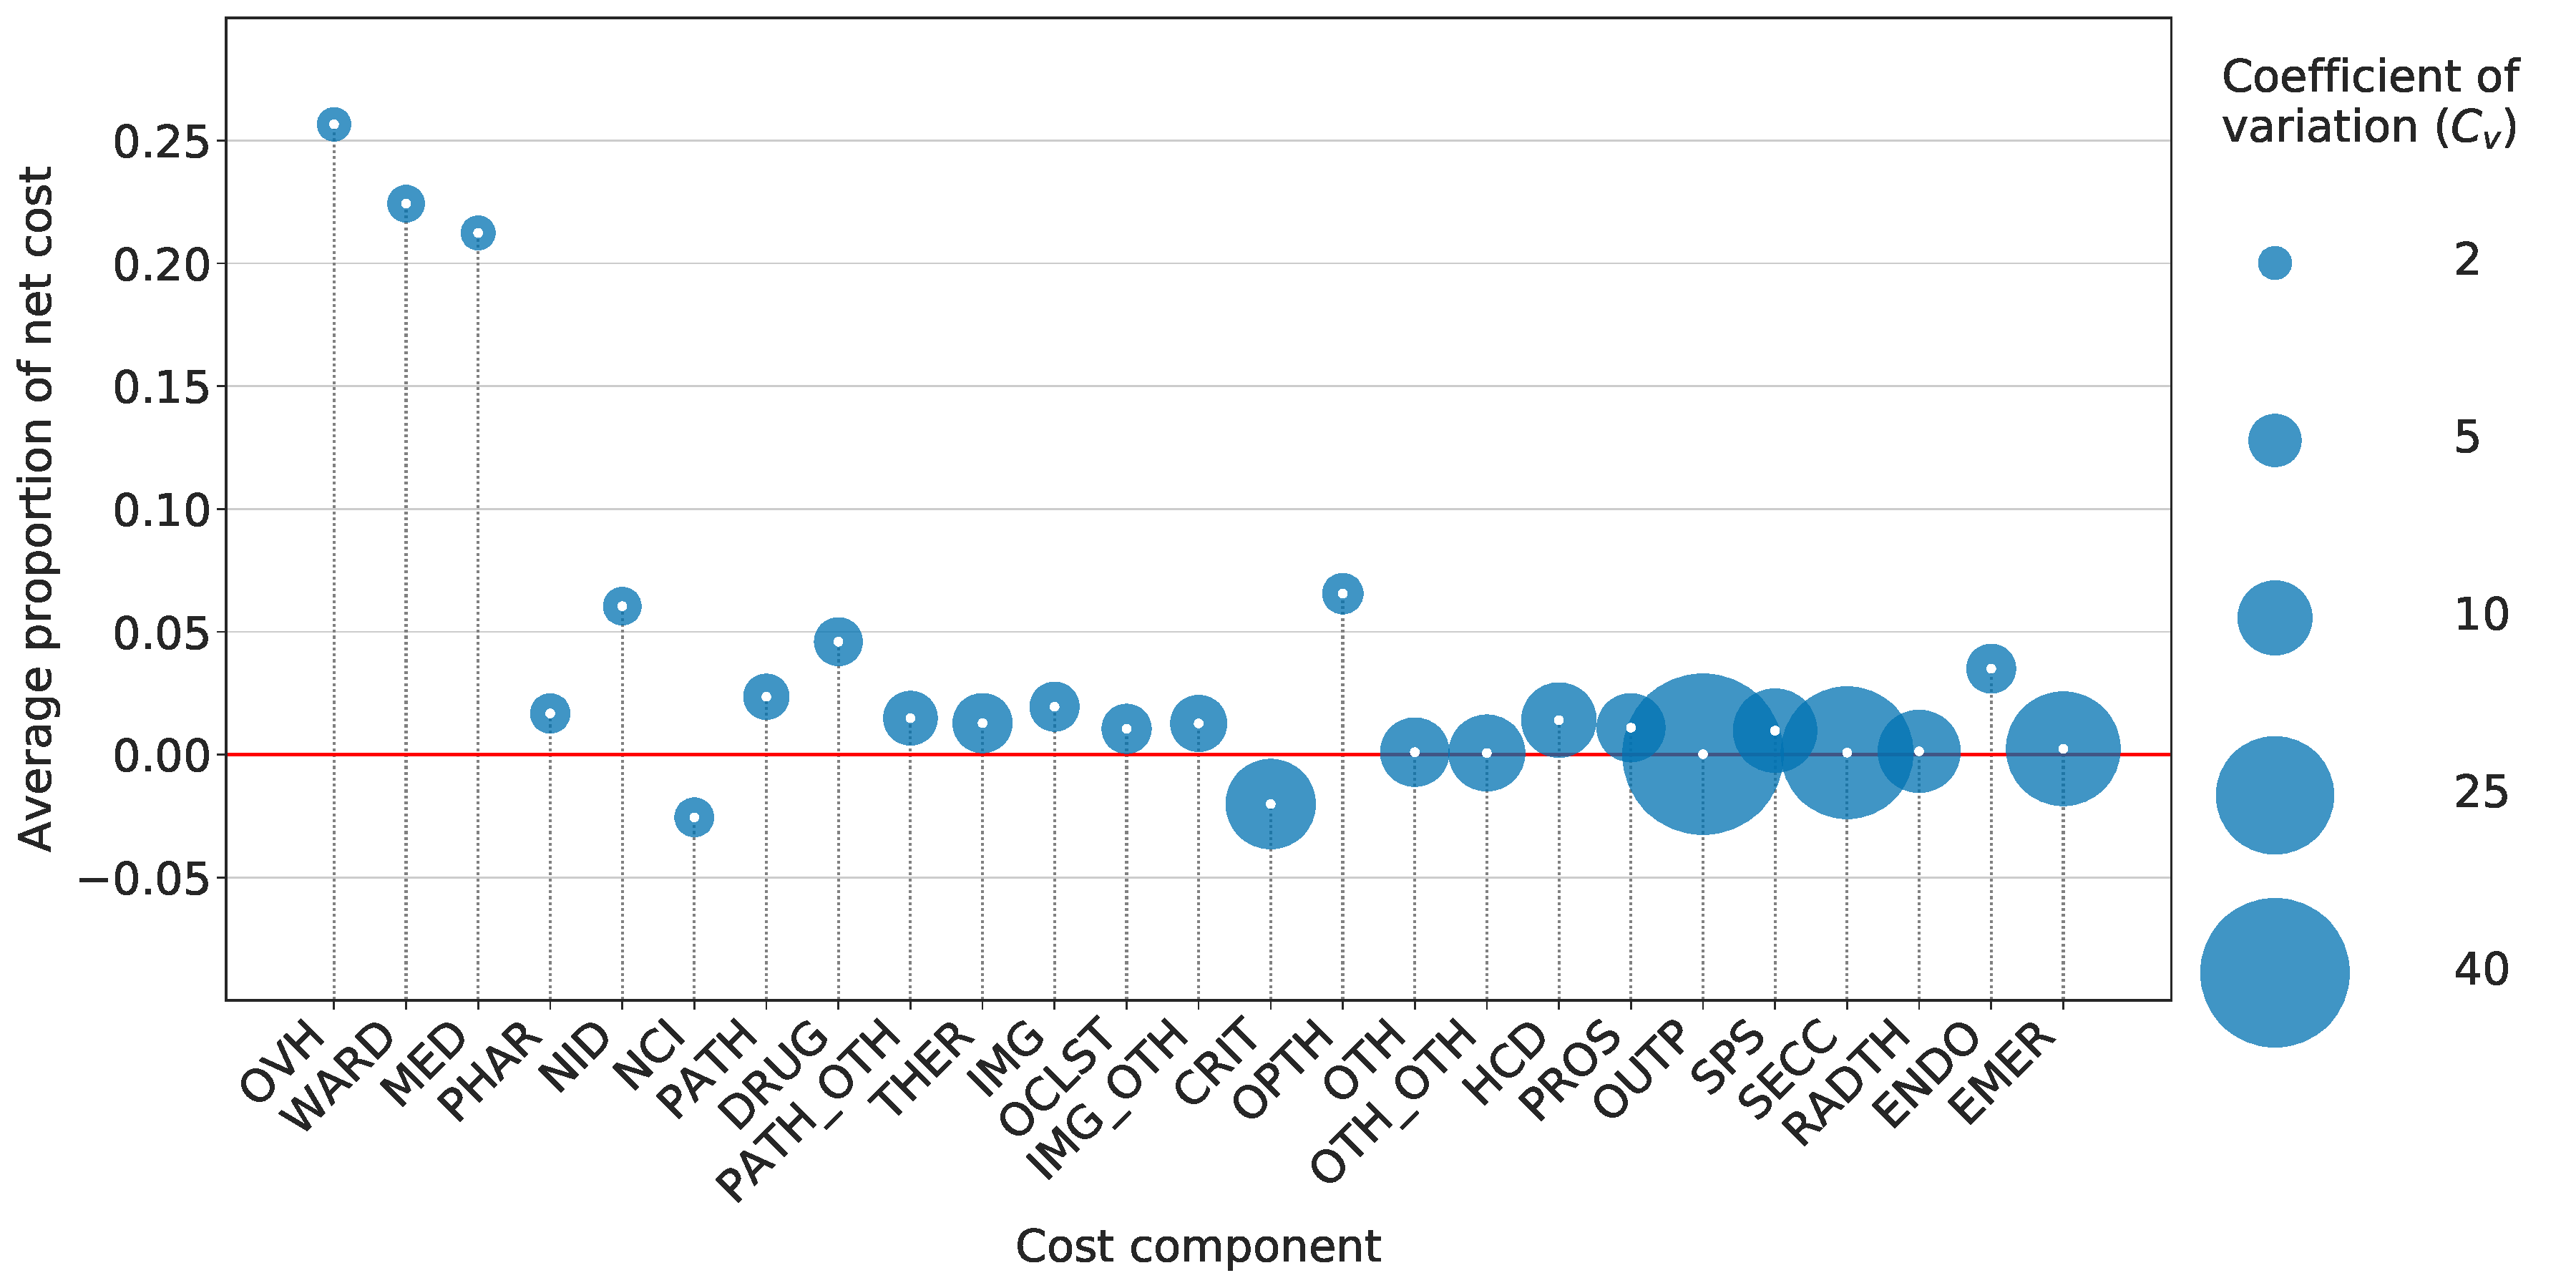
\includegraphics[width=\linewidth]{cost_bubble.pdf}
}


\section{Diabetic patient analysis}
\graphicspath{{img/diabetes/}}
\frame{\frametitle{Diabetic overview}
    \begin{minipage}{.5\linewidth}
        \makebox[\linewidth]{%
            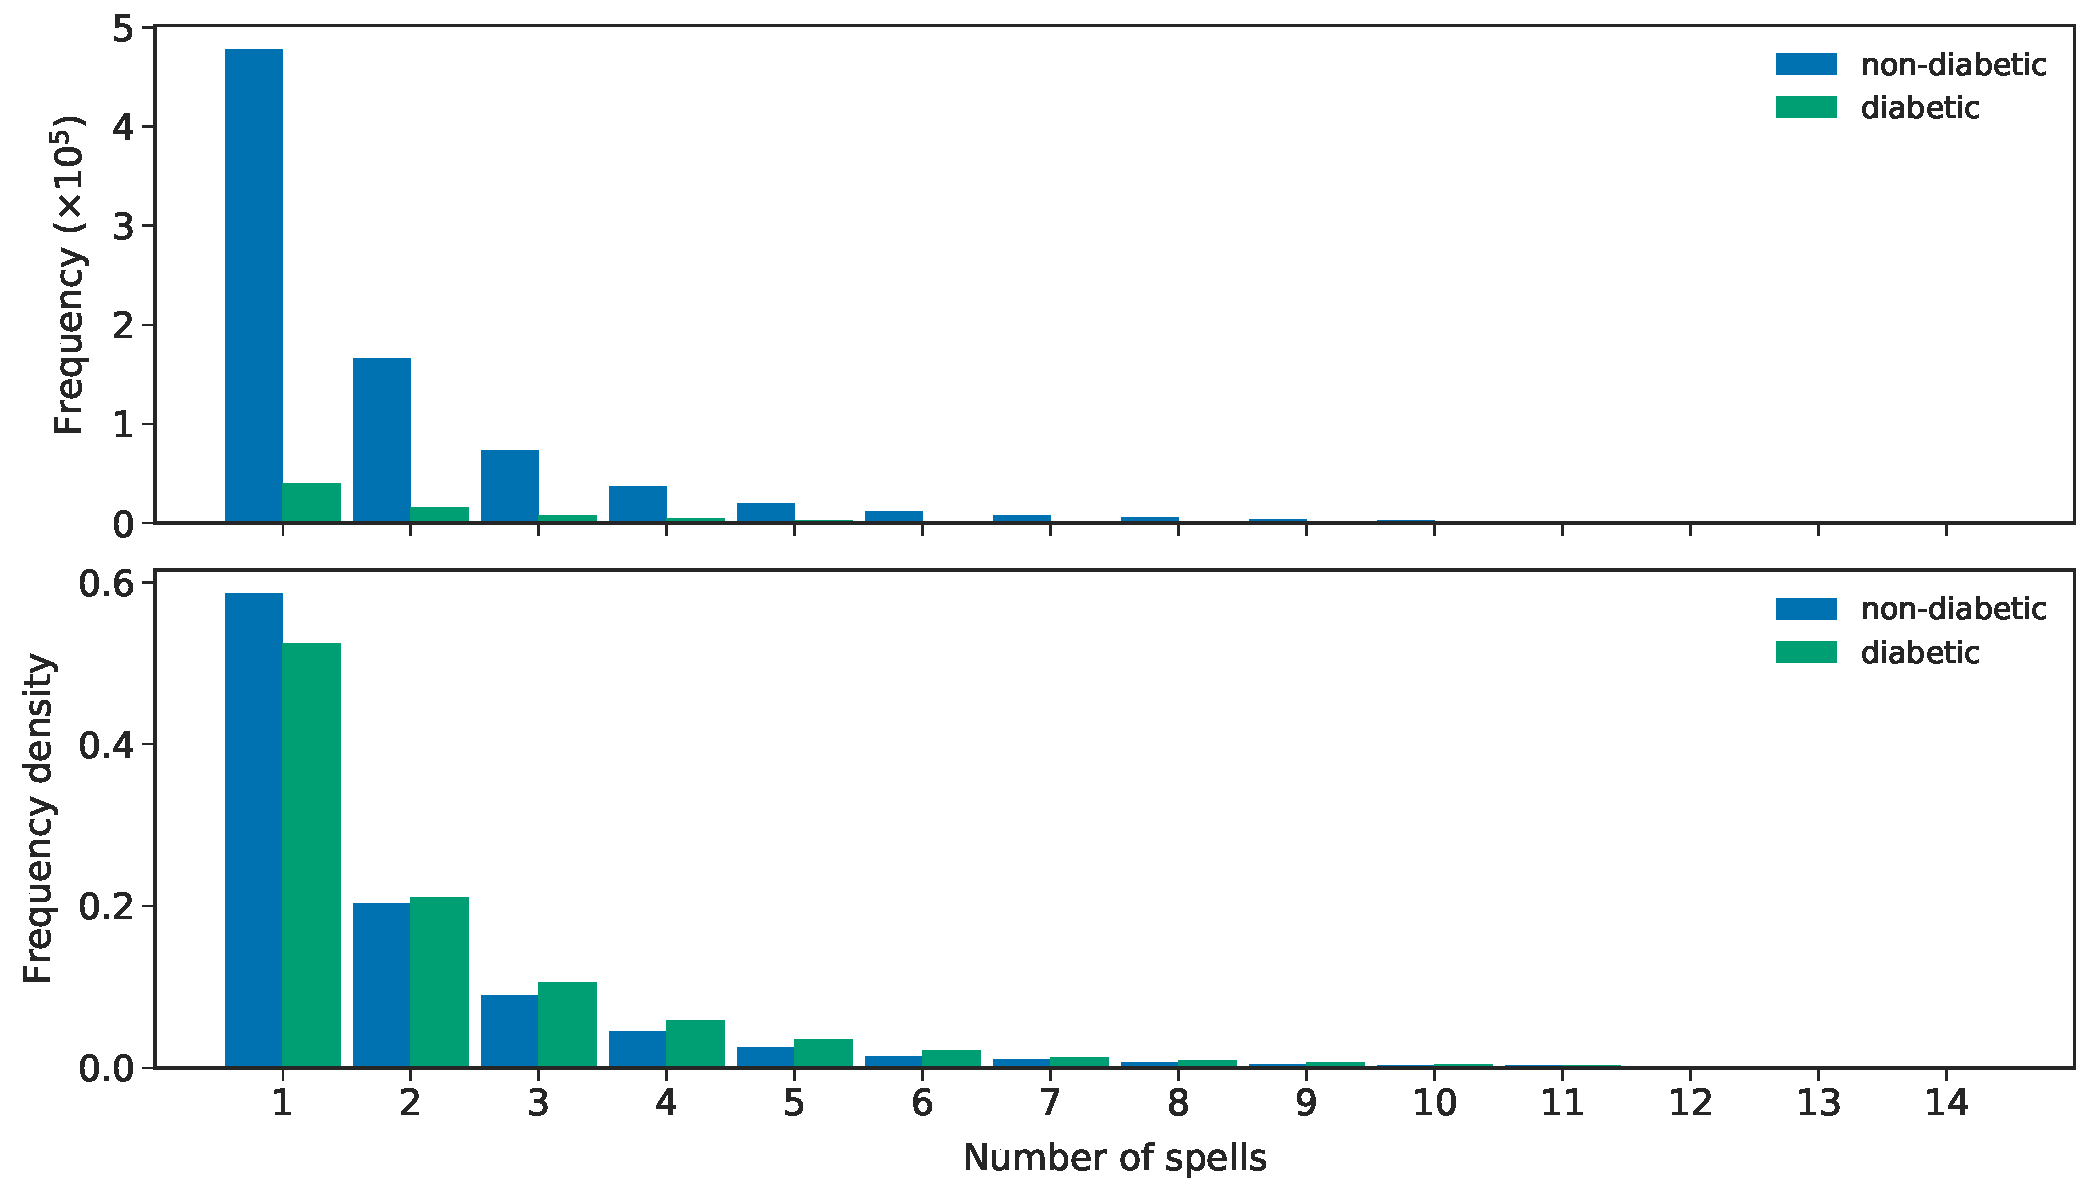
\includegraphics[width=\linewidth]{nspells_bar.pdf}
        }
    \end{minipage}%
    \begin{minipage}{.5\linewidth}
        \makebox[\linewidth]{%
            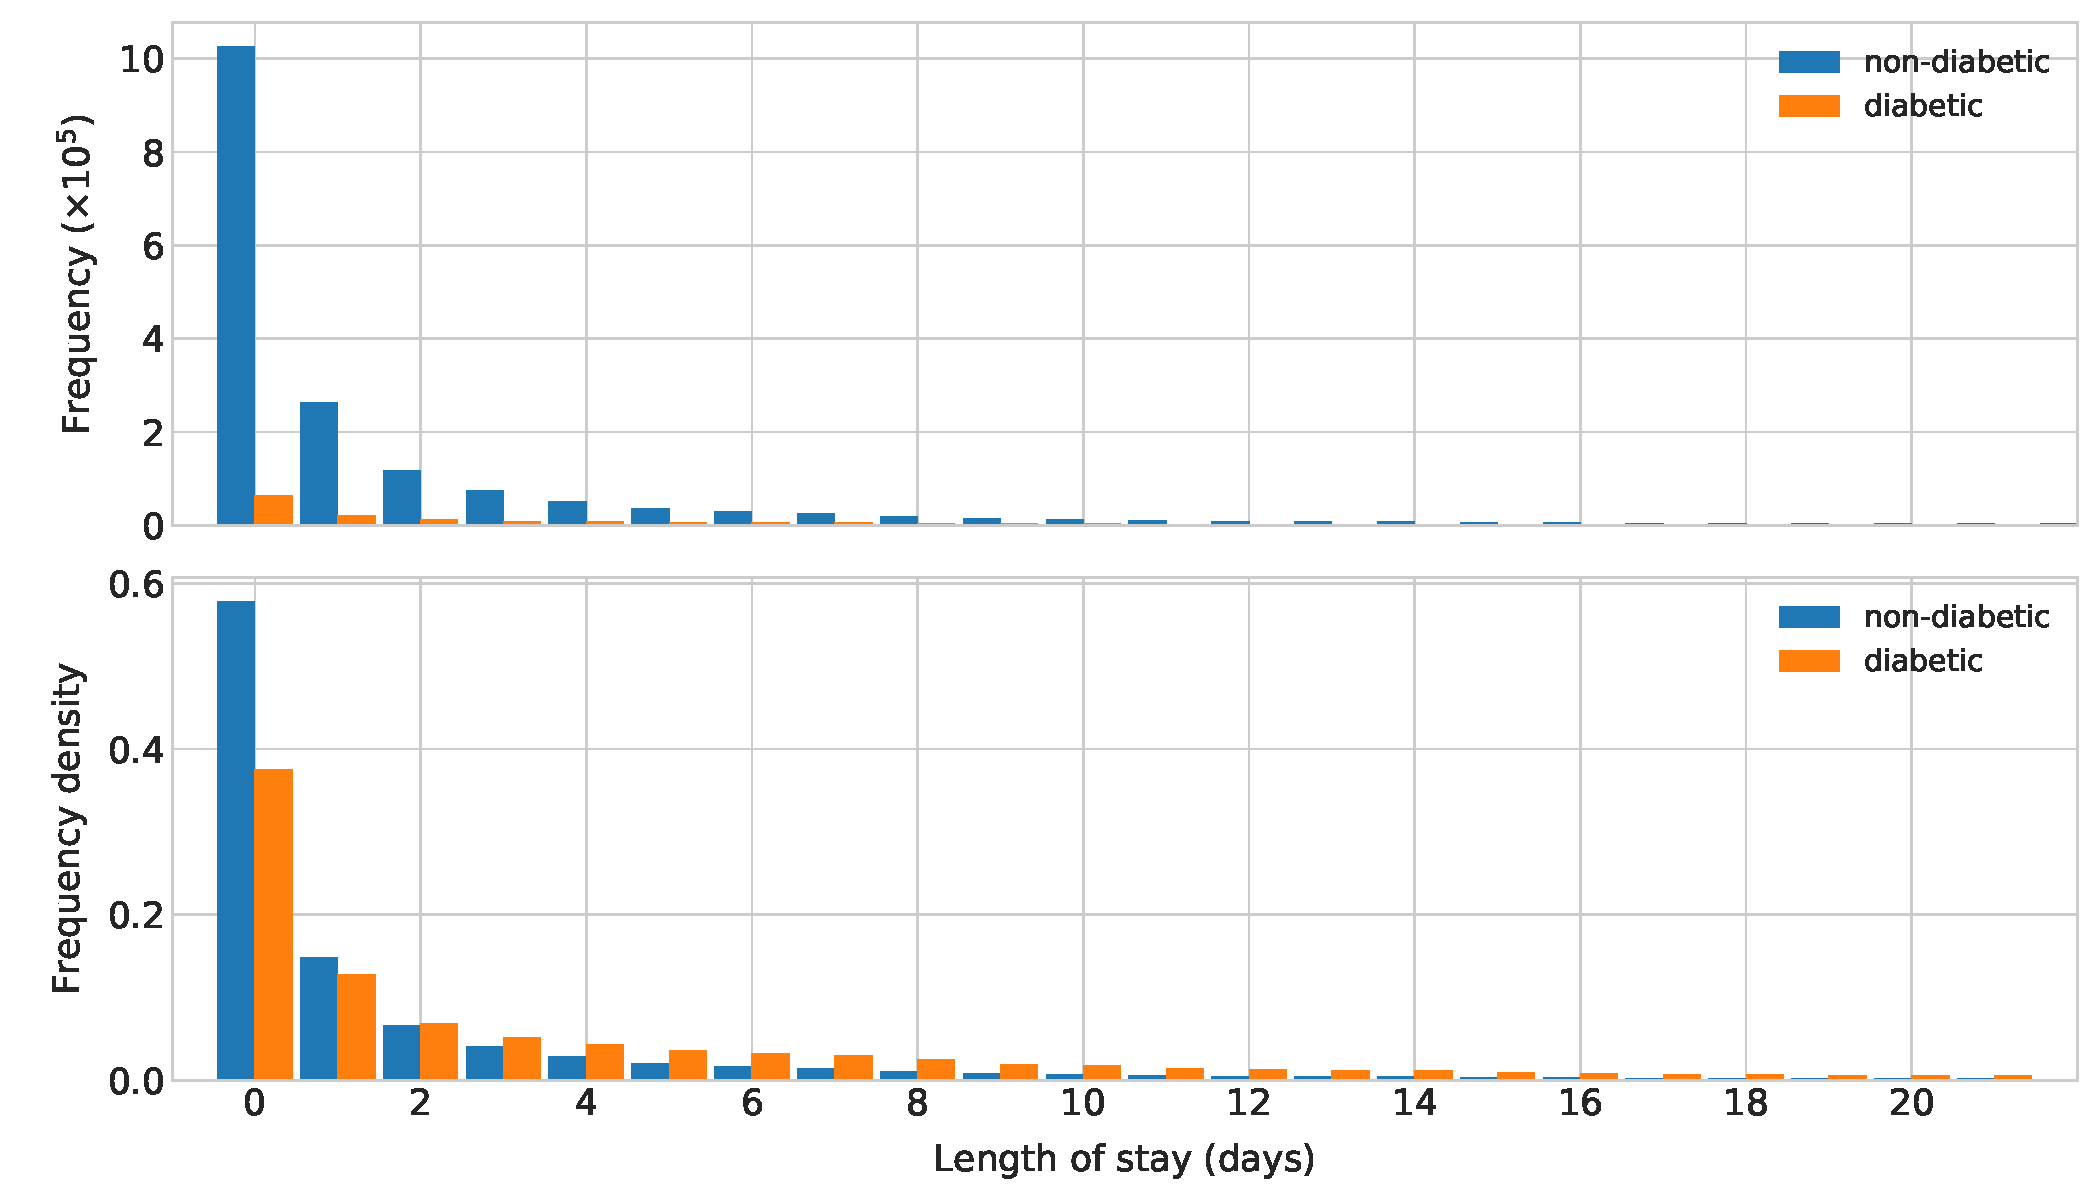
\includegraphics[width=\linewidth]{los_bar.pdf}
        }
    \end{minipage}

    \begin{minipage}{.5\linewidth}
        \makebox[\linewidth]{%
            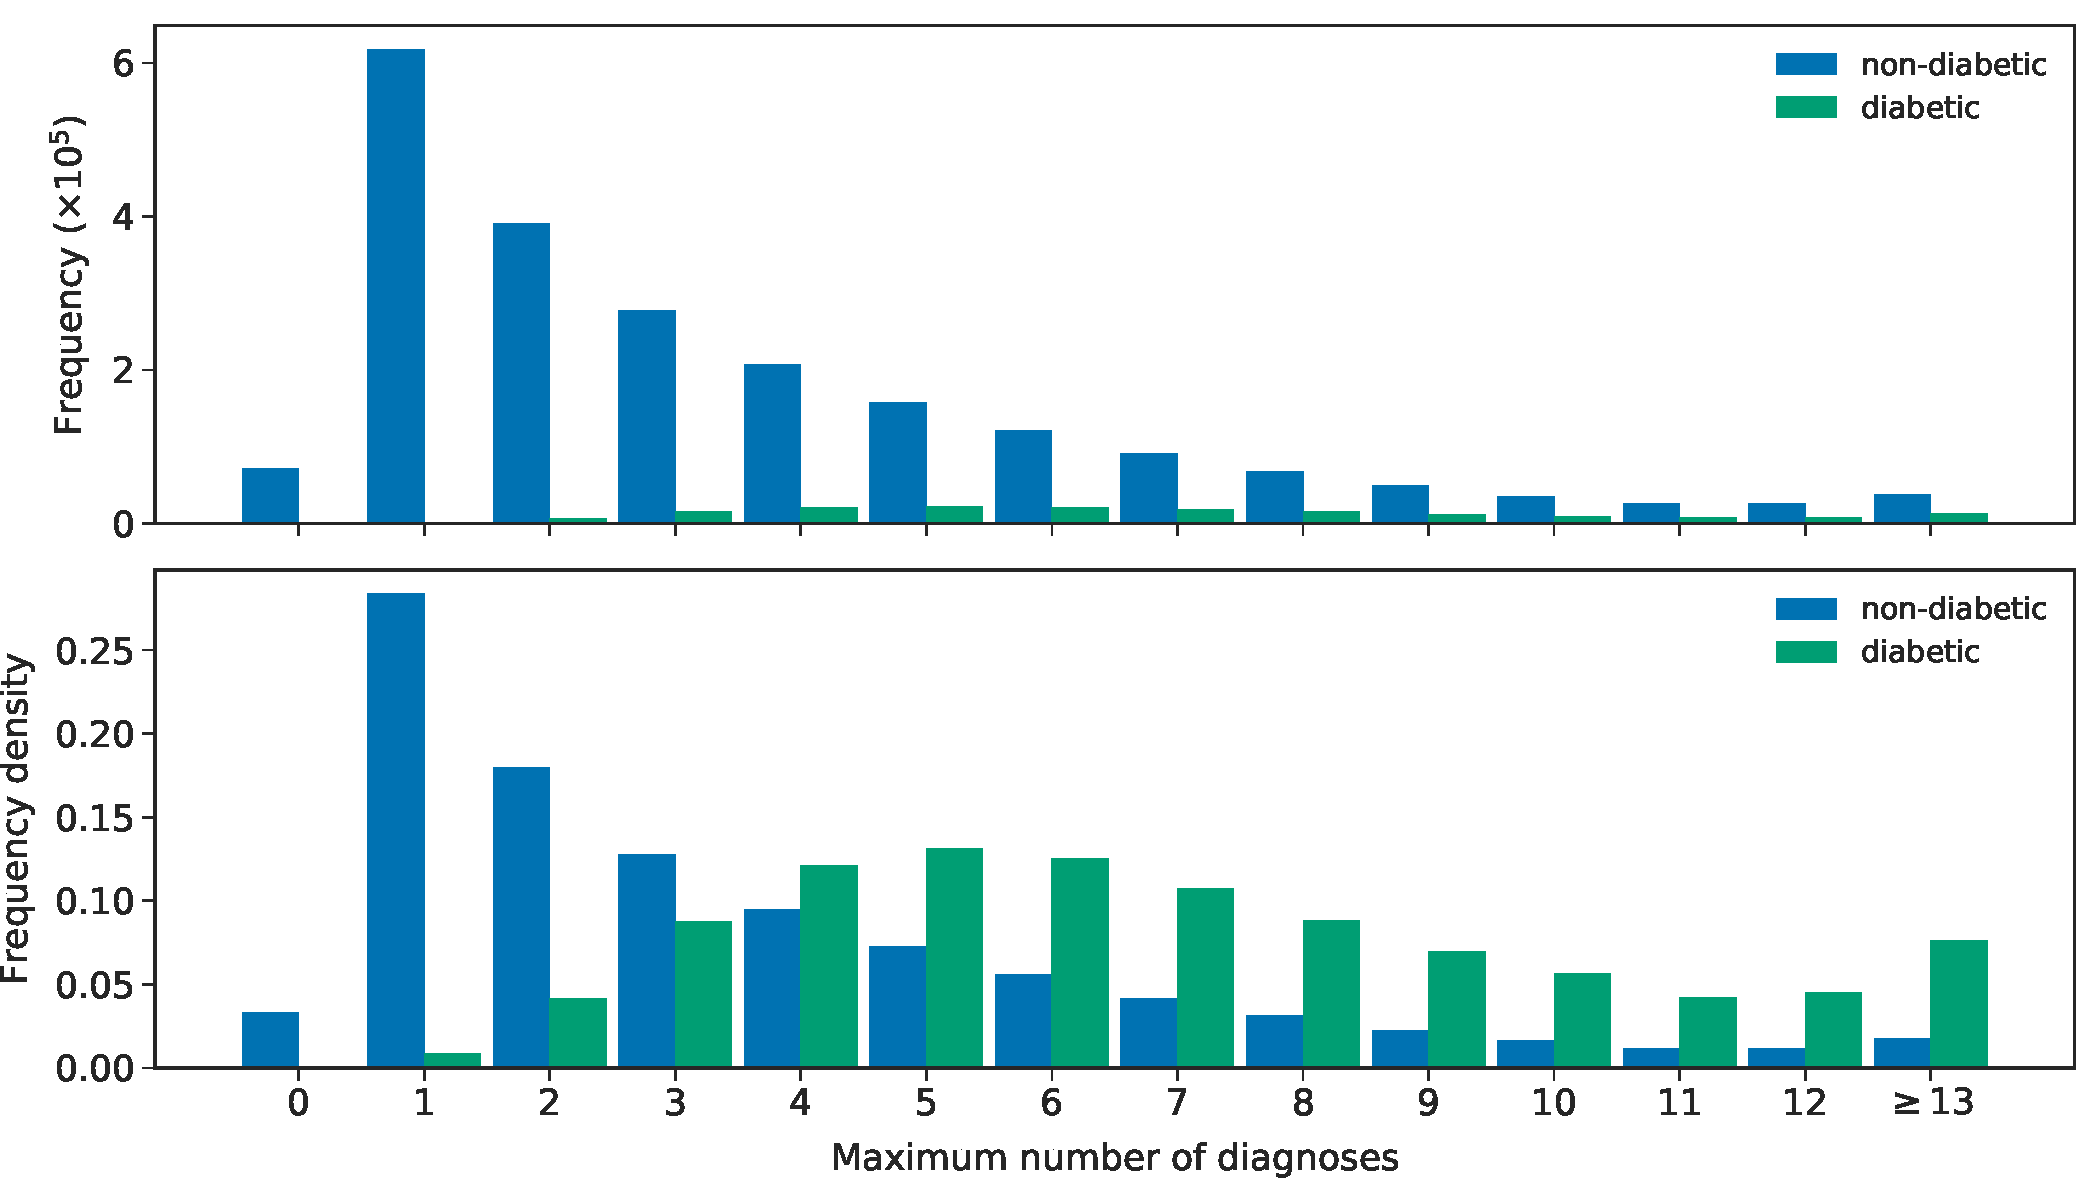
\includegraphics[width=\linewidth]{ndiag_bar.pdf}
        }
    \end{minipage}%
    \begin{minipage}{.5\linewidth}
        \makebox[\linewidth]{%
            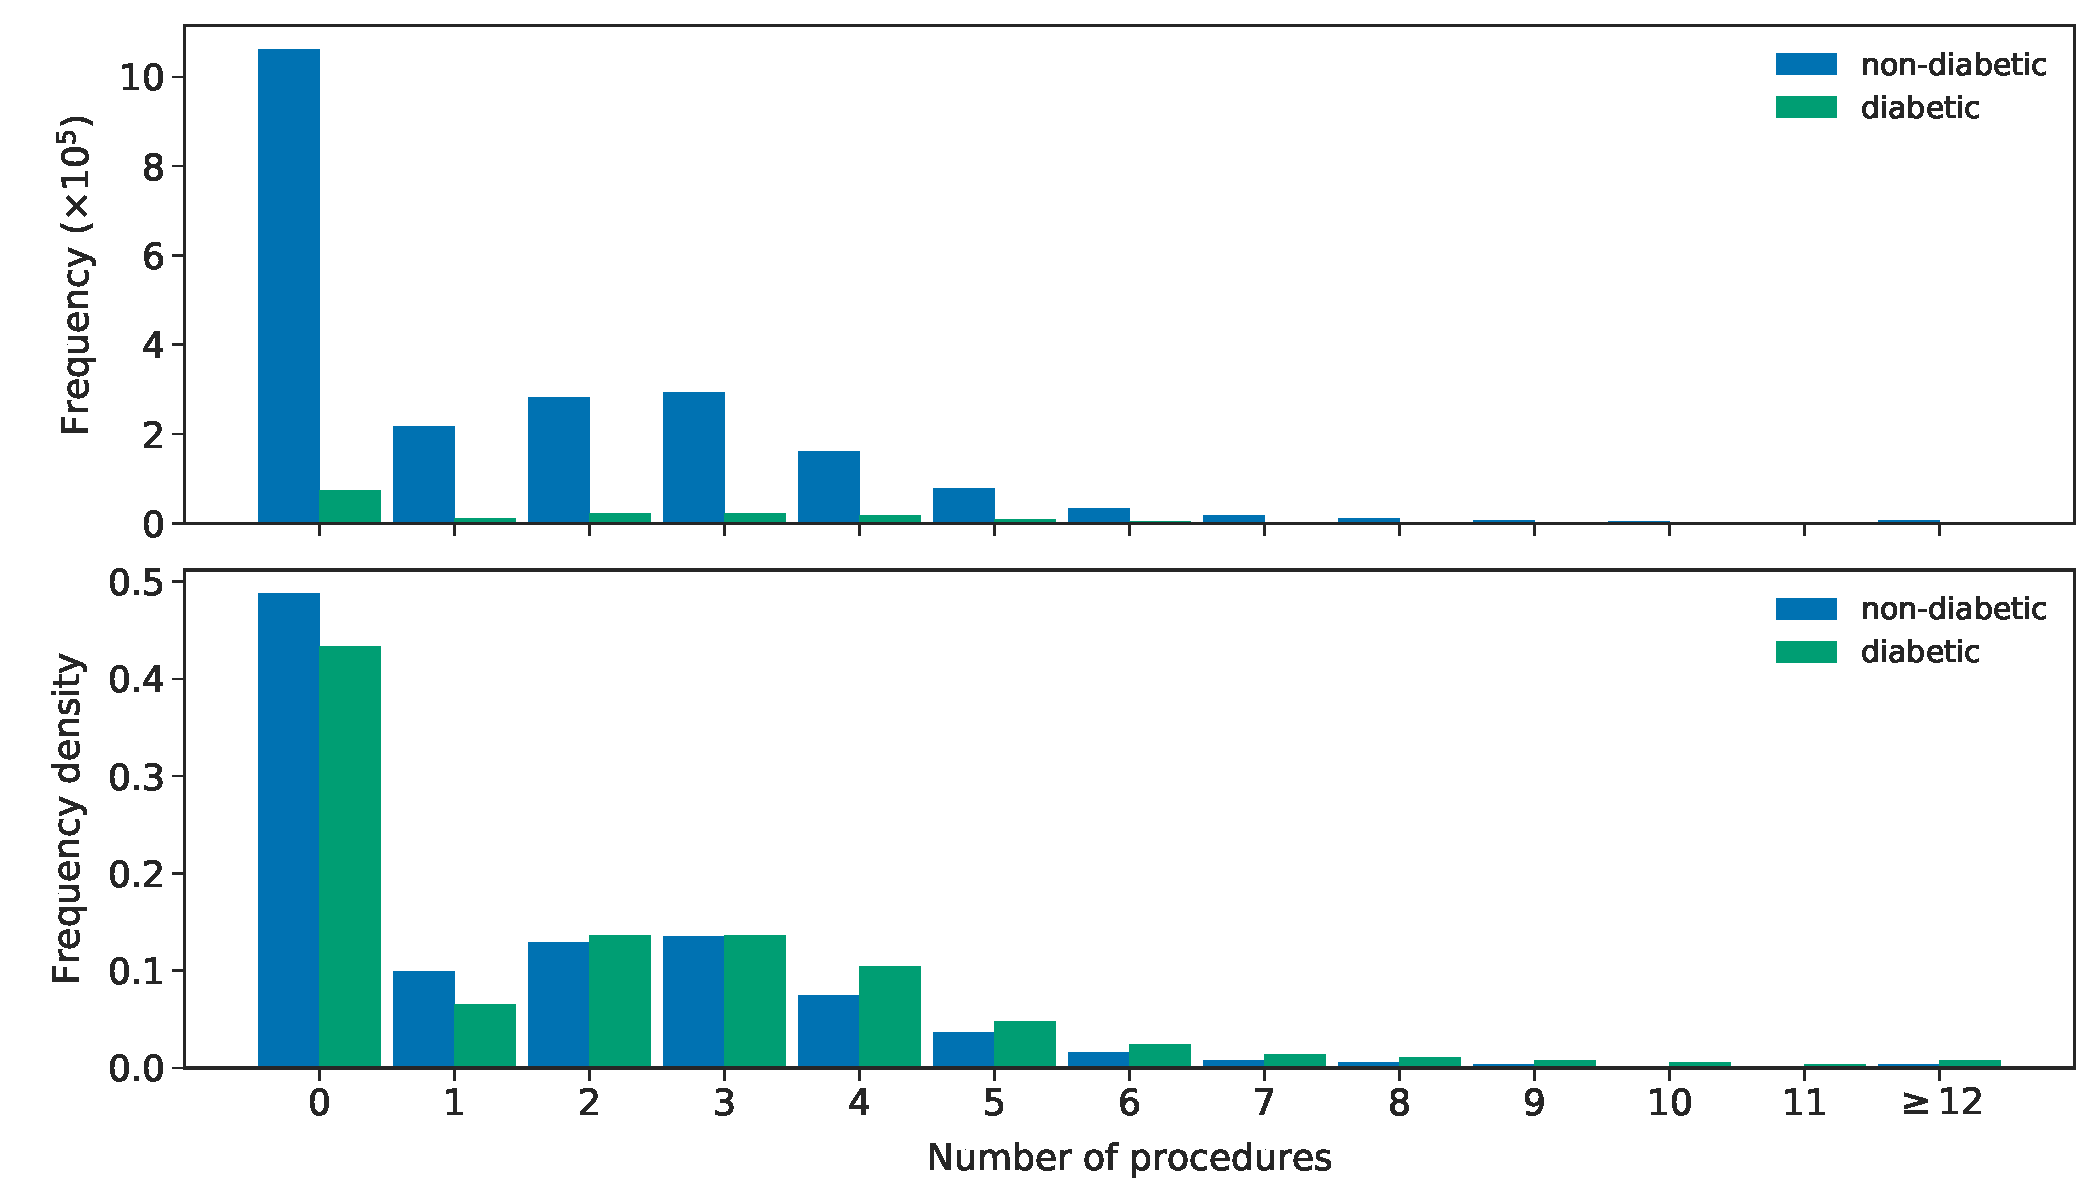
\includegraphics[width=\linewidth]{nproc_bar.pdf}
        }
    \end{minipage}
}

\frame{\frametitle{An overview}
    \makebox[\linewidth]{%
        \begin{minipage}{.8\imgwidth}
            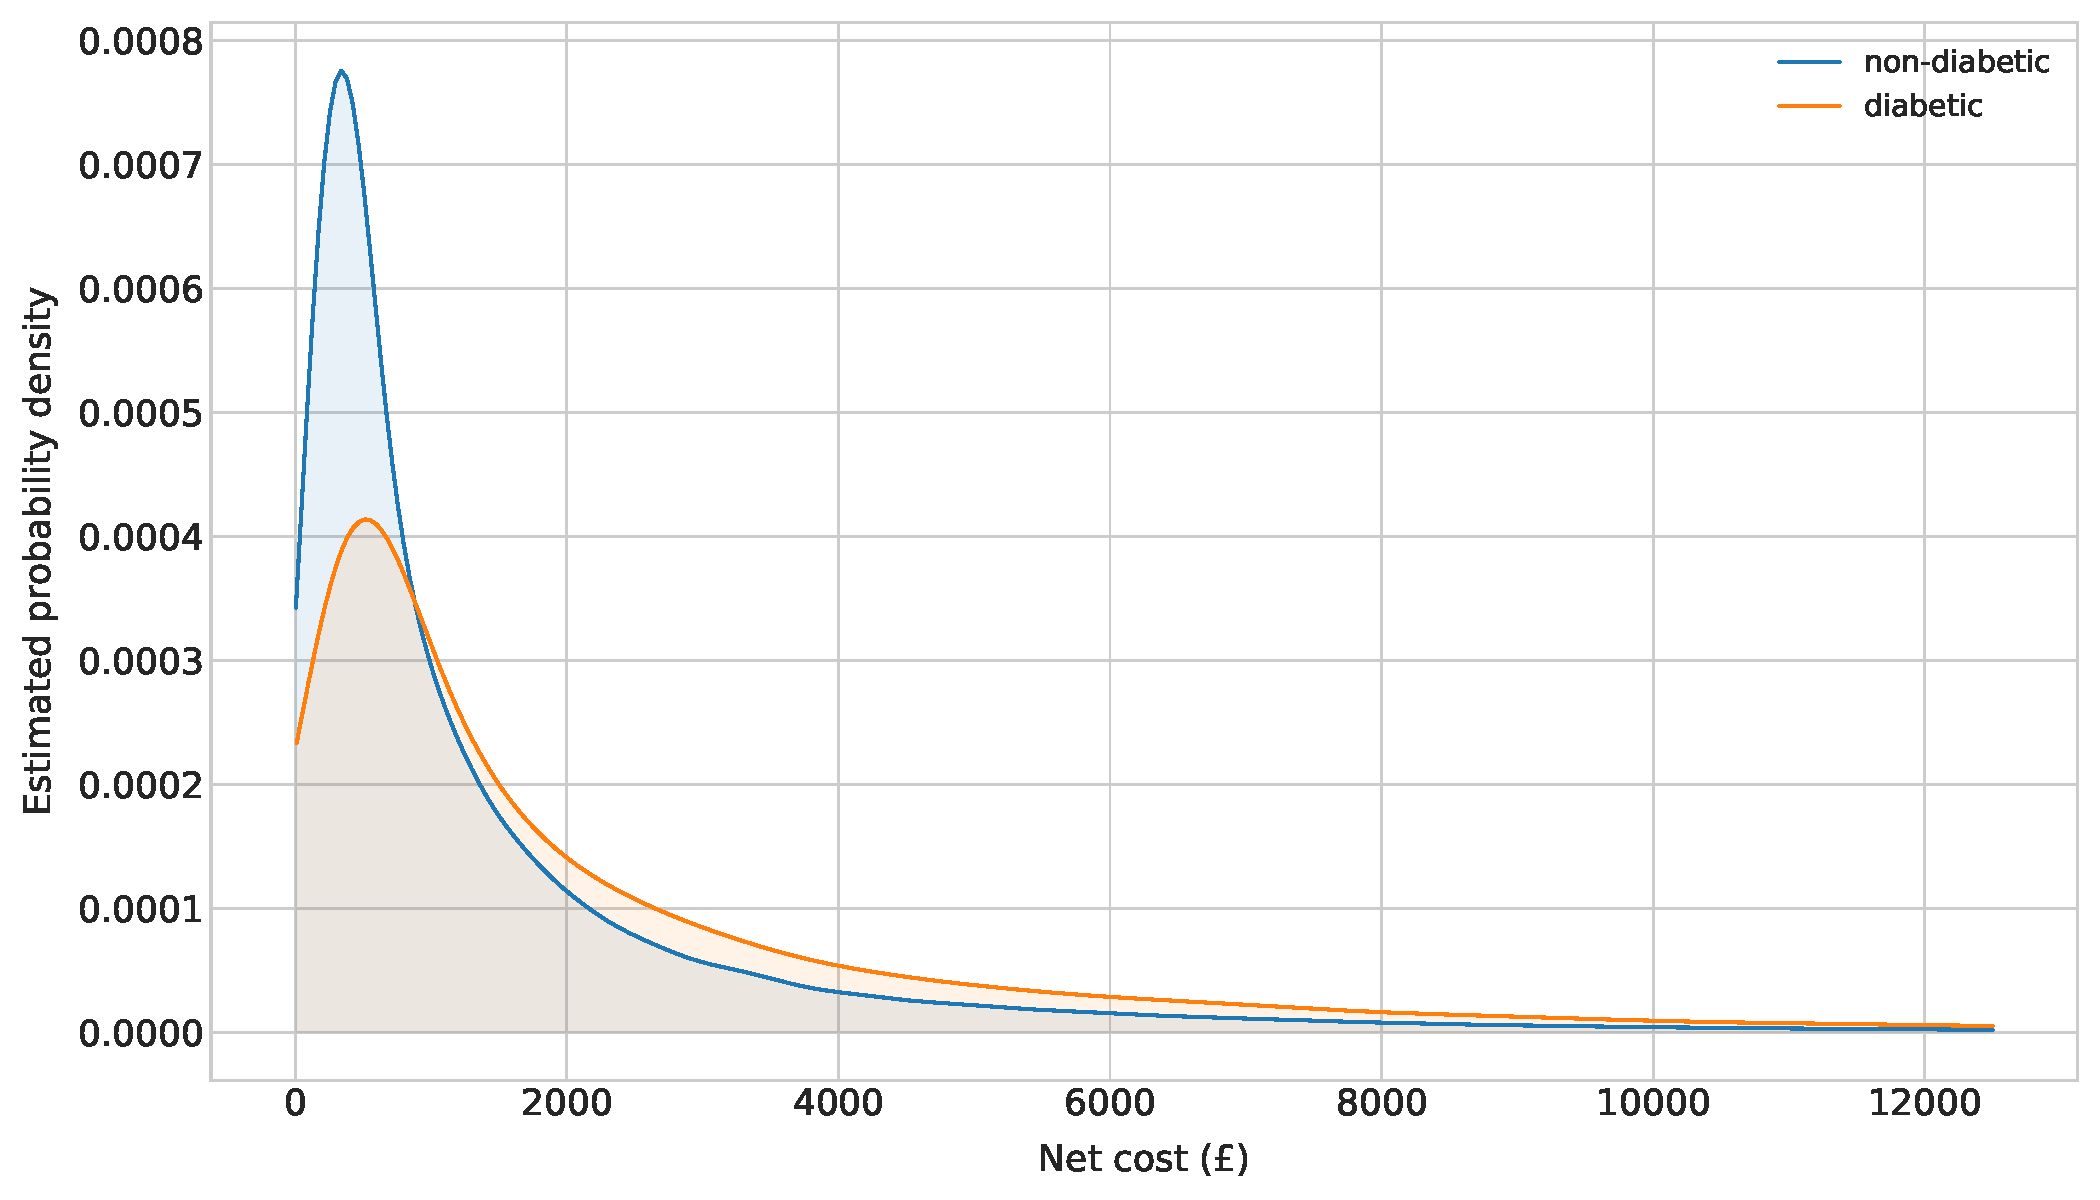
\includegraphics[width=\linewidth]{netcost_kde.pdf}
        \end{minipage}%
        \begin{minipage}{.2\paperwidth}
            \resizebox{\linewidth}{!}{%
                \begin{tabular}{lll}
\toprule
{} & Non-diabetic &    Diabetic \\
\midrule
mean &     1,647.01 &    2,648.98 \\
std  &     3,019.54 &    4,152.20 \\
min  &         4.50 &       10.91 \\
1\%   &        62.55 &      139.65 \\
25\%  &       338.67 &      490.64 \\
50\%  &       709.33 &    1,227.95 \\
75\%  &     1,756.90 &    3,106.44 \\
95\%  &     6,179.92 &    9,591.06 \\
99\%  &    13,414.47 &   19,128.45 \\
max  &   369,168.93 &  273,450.30 \\
\bottomrule
\end{tabular}

            }
        \end{minipage}
    }
}

\frame{\frametitle{An overview}
    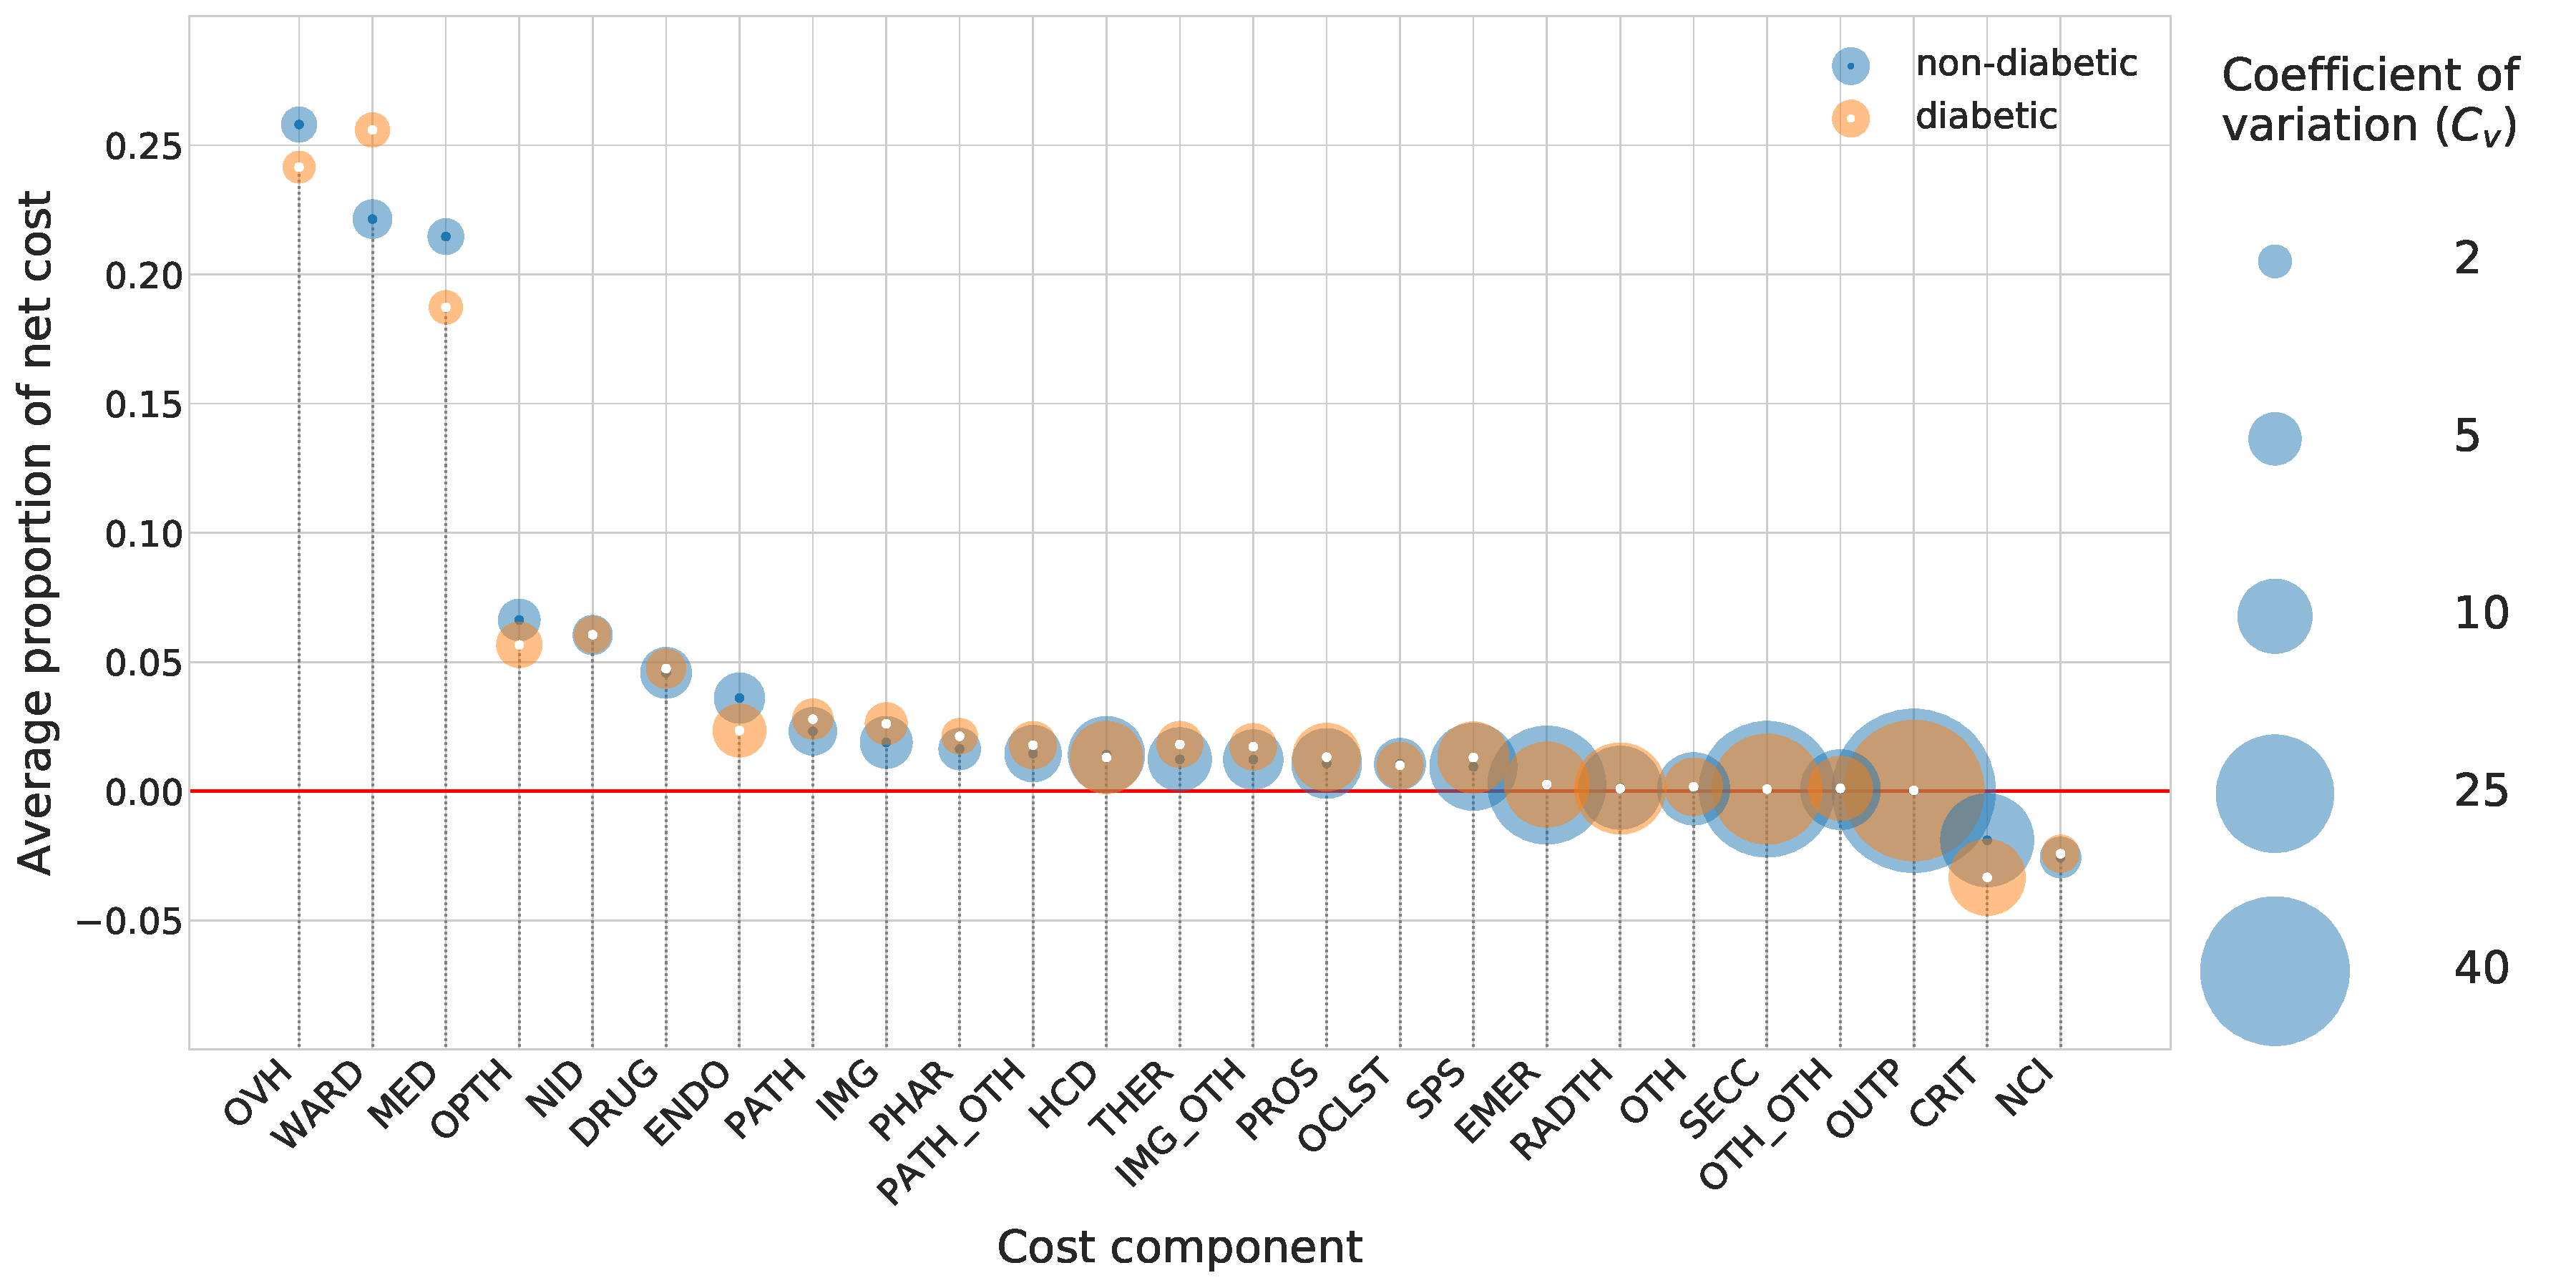
\includegraphics[width=\linewidth]{cost_bubble.pdf}
}


\end{document}
